\documentclass[a4,useAMS,usenatbib,usegraphicx]{mn2e} 
%\documentclass{latex/emulateapj} 
%External Packages and personalized macros
%=========================================================================
%		EXTERNAL PACKAGES
%=========================================================================
\usepackage{amsmath} 
\usepackage{amssymb} 
%\usepackage[section]{placeins}
\usepackage {graphicx}
%\usepackage{graphics}
\usepackage[dvips]{epsfig}
\usepackage{epsfig}  
\usepackage{color}
\usepackage[normalem]{ulem}
\usepackage{hyperref}
\usepackage{caption}
%Non reposionated tables
\usepackage{float}
\restylefloat{table}
%Multiple columns support for tables
\usepackage{array}
\usepackage{booktabs}
\setlength{\heavyrulewidth}{1.5pt}
\setlength{\abovetopsep}{4pt}
\pdfminorversion=5

%=========================================================================
%		INTERNAL MACROS
%=========================================================================
\def\be{\begin{equation}}
\def\ee{\end{equation}}
\def\ba{\begin{eqnarray}}
\def\ea{\end{eqnarray}}

% To highlight comments 
\definecolor{red}{rgb}{1,0.0,0.0}
\newcommand{\red}{\color{red}}
\definecolor{darkgreen}{rgb}{0.0,0.5,0.0}
\newcommand{\SRK}[1]{\textcolor{darkgreen}{\bf SRK: \textit{#1}}}
\newcommand{\SRKED}[1]{\textcolor{darkgreen}{\bf #1}}
\newcommand{\before}[1]{\textcolor{red}{ #1}}
\newcommand{\after}[1]{\textcolor{darkgreen}{ #1}}

\newcommand{\LCDM}{$\Lambda$CDM~}
\newcommand{\beq}{\begin{eqnarray}}  
\newcommand{\eeq}{\end{eqnarray}}  
\newcommand{\zz}{$z\sim 3$} 
\newcommand{\apj}{ApJ}  
\newcommand{\jcap}{JCAP}  
\newcommand{\apjs}{ApJS}  
\newcommand{\apjl}{ApJL}  
\newcommand{\aj}{AJ}  
\newcommand{\mnras}{MNRAS}  
\newcommand{\mnrassub}{MNRAS accepted}  
\newcommand{\aap}{A\&A}  
\newcommand{\aaps}{A\&AS}  
\newcommand{\araa}{ARA\&A}  
\newcommand{\nat}{Nature}  
\newcommand{\physrep}{PhR}
\newcommand{\pasp}{PASP}    
\newcommand{\pasj}{PASJ}    
\newcommand{\avg}[1]{\langle{#1}\rangle}  
\newcommand{\ly}{{\ifmmode{{\rm Ly}\alpha}\else{Ly$\alpha$}\fi}}
\newcommand{\hMpc}{{\ifmmode{h^{-1}{\rm Mpc}}\else{$h^{-1}$Mpc}\fi}}  
\newcommand{\hGpc}{{\ifmmode{h^{-1}{\rm Gpc}}\else{$h^{-1}$Gpc}\fi}}  
\newcommand{\hmpc}{{\ifmmode{h^{-1}{\rm Mpc}}\else{$h^{-1}$Mpc}\fi}}  
\newcommand{\hkpc}{{\ifmmode{h^{-1}{\rm kpc}}\else{$h^{-1}$kpc}\fi}}  
\newcommand{\hMsun}{{\ifmmode{h^{-1}{\rm {M_{\odot}}}}\else{$h^{-1}{\rm{M_{\odot}}}$}\fi}}  
\newcommand{\hmsun}{{\ifmmode{h^{-1}{\rm {M_{\odot}}}}\else{$h^{-1}{\rm{M_{\odot}}}$}\fi}}  
\newcommand{\Msun}{{\ifmmode{{\rm {M_{\odot}}}}\else{${\rm{M_{\odot}}}$}\fi}}  
\newcommand{\msun}{{\ifmmode{{\rm {M_{\odot}}}}\else{${\rm{M_{\odot}}}$}\fi}}  
\newcommand{\lya}{{Lyman$\alpha$~}}
\newcommand{\clara}{{\texttt{CLARA}}~}
\newcommand{\rand}{{\ifmmode{{\mathcal{R}}}\else{${\mathcal{R}}$ }\fi}}  
%SAMPLES
\newcommand{\GHBDM}{\texttt{GH}$_{\mbox{\tiny{BDM}}}$ }
\newcommand{\GHFOF}{\texttt{GH}$_{\mbox{\tiny{FOF}}}$ }
\newcommand{\IHBDM}{\texttt{IH}$_{\mbox{\tiny{BDM}}}$ }
\newcommand{\IHFOF}{\texttt{IH}$_{\mbox{\tiny{FOF}}}$ }
\newcommand{\PBDM}{\texttt{P}$_{\mbox{\tiny{BDM}}}$ }
\newcommand{\PFOF}{\texttt{P}$_{\mbox{\tiny{FOF}}}$ }
\newcommand{\IPBDM}{\texttt{IP}$_{\mbox{\tiny{BDM}}}$ }
\newcommand{\IPFOF}{\texttt{IP}$_{\mbox{\tiny{FOF}}}$ }
\newcommand{\RIPBDM}{\texttt{RIP}$_{\mbox{\tiny{BDM}}}$ }
\newcommand{\RIPFOF}{\texttt{RIP}$_{\mbox{\tiny{FOF}}}$ }


%MY COMMANDS #############################################################
\newcommand{\sub}[1]{\mbox{\scriptsize{#1}}}
\newcommand{\dtot}[2]{ \frac{ d #1 }{d #2} }
\newcommand{\dpar}[2]{ \frac{ \partial #1 }{\partial #2} }
\newcommand{\pr}[1]{ \left( #1 \right) }
\newcommand{\corc}[1]{ \left[ #1 \right] }
\newcommand{\lla}[1]{ \left\{ #1 \right\} }
\newcommand{\bds}[1]{\boldsymbol{ #1 }}
\newcommand{\oiint}{\displaystyle\bigcirc\!\!\!\!\!\!\!\!\int\!\!\!\!\!\int}
\newcommand{\mathsize}[2]{\mbox{\fontsize{#1}{#1}\selectfont $#2$}}
\newcommand{\eq}[2]{\begin{equation} \label{eq:#1} #2 \end{equation}}
\newcommand{\lth}{$\lambda_{th}$ }
\newcommand{\reff}{{\ifmmode{r_{\mbox{\tiny eff}}}\else{$r_{\mbox{\tiny eff}}$}\fi}}
%#########################################################################

\begin{document}

%=========================================================================
%		FRONT MATTER
%=========================================================================
\title[]{The environmental effect on the neutral column density of
LAEs at $z\sim 6$}
%\author[C.N. Poveda-Ruiz, J.E. Forero-Romero, J.C. Mu\~noz-Cuartas]{
%\parbox[t]{\textwidth}{\raggedright 
%  C. N. Poveda-Ruiz \thanks{cn.poveda542@uniandes.edu.co}$^{1}$
%  J. E. Forero-Romero \thanks{je.forero@uniandes.edu.co}$^{1}$
%  J. C. Mu\~noz-Cuartas \thanks{juan.munozc@udea.edu.co}$^{2}$
%}
%\vspace*{6pt}\\
%$^1$Departamento de F\'{i}sica, Universidad de los Andes, Cra. 1
%No. 18A-10, Edificio Ip, Bogot\'a, Colombia\\
%$^2$Instituto de F\'{\i}sica - FCEN, Universidad de Antioquia, Calle
%67 No. 53-108, Medell\'{\i}n, Colombia
%}

\maketitle

\begin{abstract}
\end{abstract}

\begin{keywords}
\end{keywords}


%*************************************************************************
\section{Introduction}
\label{sec:introduction}
%*************************************************************************



\section{Analytic derivations:}
\subsection{Gas density profile:}\label{sec:rho}

Assuming that the Hydrogen is in isothermal \citep{Makino98} derive an 
analytical expression for the Hydrogen gas profile inside a
Navarro-Frenk-White Dark Matter halo:

\begin{equation}\label{eq:rhogr}
\rho_g(r) =  \dfrac{\rho_{g,0}A}{\left[ 1 + \left(\dfrac{r}{r_{c,eff}}\right)^2 \right]^{3\beta_{eff}/2}}
\end{equation}

Where $A(b) = -0.178b + 0.982$, $\beta_{eff} = 0.9 b$, $r_{c, eff}=
0.22 r_s$ ($r_s$ is the NFW scale length) and $\rho_{g,0}$ is defined
as:

\begin{equation}\label{eq:rhog0}
\rho_{g0} =\dfrac{f_g\Omega_{b}\rho_{c0}\delta_{c}}{\Omega_0}e^{27b/2} \left
[Ln(1+c) - \dfrac{c}{1+c} \right] \left [ \int_0^c x^2(1+x)^{27b/2x} dx \right ]^{-1}
\end{equation}

As an example, for a dark matter halo of $M_{vir} = 1E12 M_{\odot}$ at
$z=2$ with $c=3.75$,  $\rho_{g,0}=1.37\times10^{-25} g/cm^{-3}$ and
the Hydrogen density profile is shown in figure.\ref{fig:gp}.

\begin{figure*}
\centering
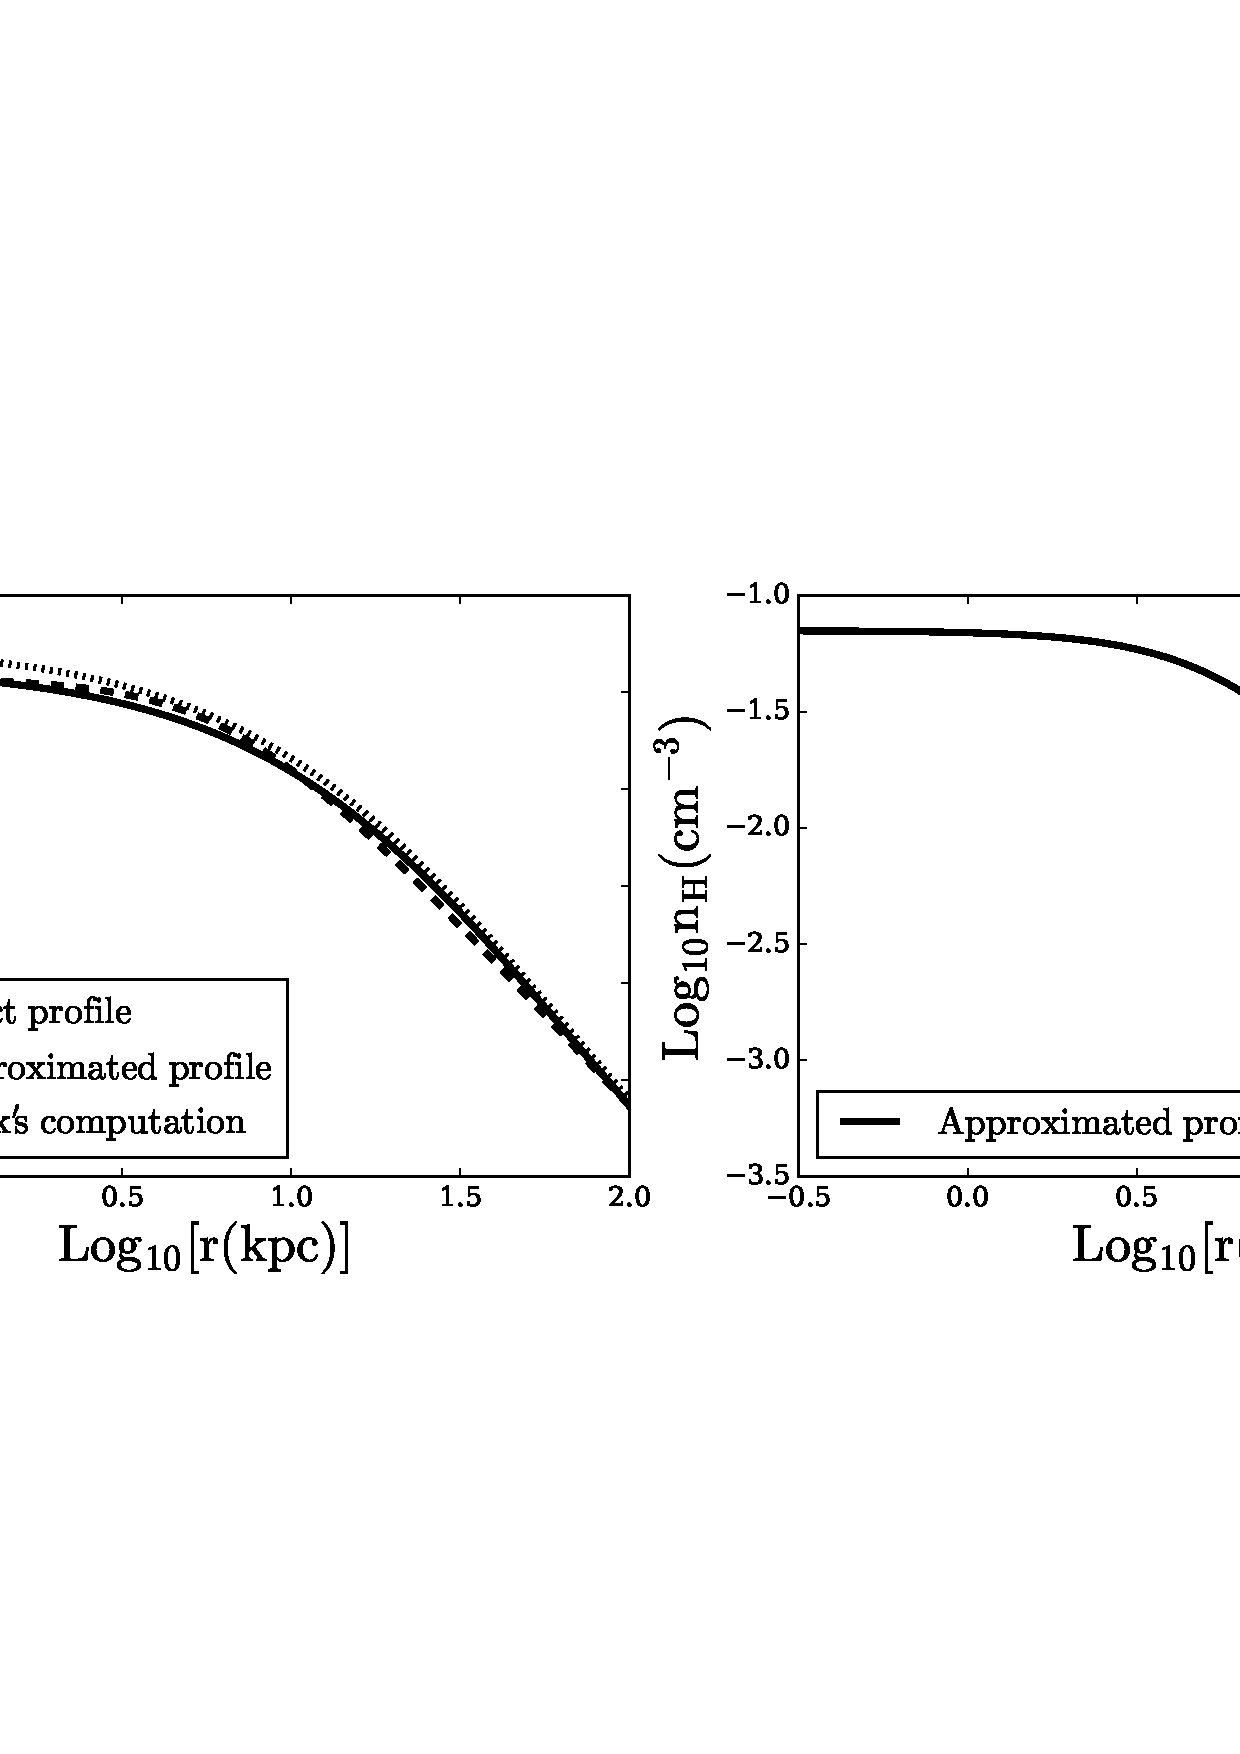
\includegraphics[scale=0.5]{../figures/gasprofile.pdf}
\caption{Gas density profile for a Dark Matter halo of $M_{vir} = 1E12
M_{\odot}$ at $z=2$ with $c=3.75$ \label{fig:gp}}
\end{figure*}


\subsection{Neutral Hydrogen column density derivation:}\label{sec:NH}

The column density $N_{H}$ of the Hydrogen is:

\begin{equation}
N_{H} = \int \limits_{-\infty}^{\infty}\rho_g(r)dz
\end{equation}

Where $r^2 = z^2 + b'^2$ and $b'$ is the impact parameter (here $z$
should not be confused with the redshift).
Which in terms of $r$ is:

\begin{equation}
N_{H} = \rho_{g0}A \int \limits_{-\infty}^{\infty} \dfrac{dz}{\left
[ 1 + \left(\dfrac{r}{r_{c,eff}} \right)^2 \right]^{3\beta_{eff}/2}}
= \rho_{g0}A \int \limits_{b}^{\infty}\dfrac{r}{\sqrt{r^2 - b'^2}}\dfrac{dr}
{\left [ 1 + \left(\dfrac{r}{r_{c,eff}} \right)^2 \right]^{3\beta_{eff}/2}}
\end{equation}

The result of the integral is:

\begin{equation}\label{eq:NH}
\begin{split}
N_{H} = \rho_{g0} A\dfrac{\sqrt{\pi} (\dfrac{1}{r_{c,eff}(M_h)^2})^{-3\beta_{eff}(M_h) /2} (b'^2 + r_{c,eff}(M_h)^2)^{1/2 - 3\beta_{eff}(M_h)/2} \Gamma(-1/2 + 3\beta_{eff}/2) }{2 \Gamma(\dfrac{3\beta_{eff}(M_h)}{2})}
\end{split}
\end{equation}


Figure \ref{fig:NHb} shows the dependence of the column density $N_H$
for different impact parameters $b'$ and different halo concentration.
\begin{figure}
\centering
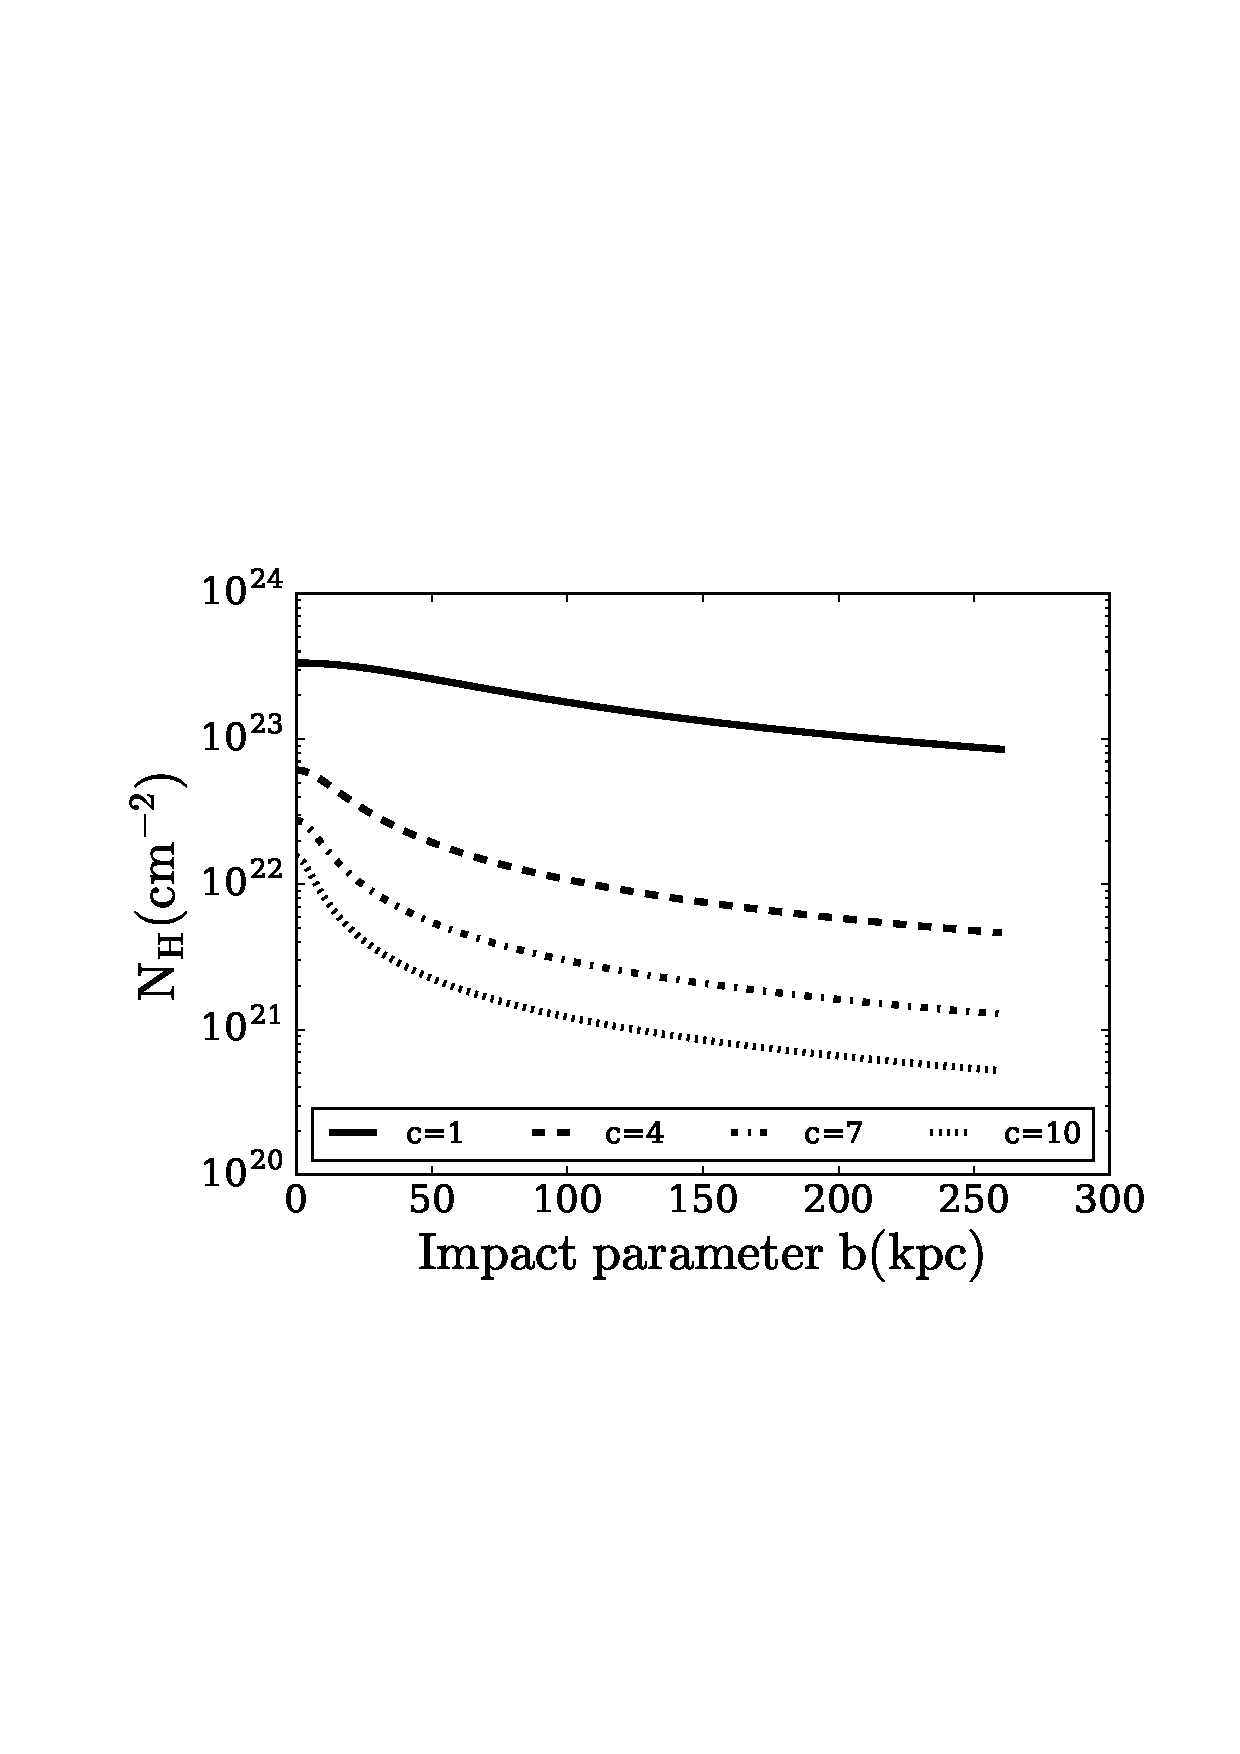
\includegraphics[scale=0.5]{../figures/NH-b.pdf}
\caption{Column density values for different values of the impact
parameter and for different halo concentrations.\label{fig:NHb}}
\end{figure}

%The average column density $N_H$ of all the halos at all the possible
%impact parameters is:

%\begin{equation}\label{eq:integral}
%<N_H> = 4 \int \limits_0^{0.5} dx \int \limits_{0}^{0.5}dy \int
%\limits_{M_{Hmin}}^{M_{Hmax}} N_H(b, M_H)\xi(M_H)dM_H
%\end{equation}

%Where the impact paremeter $b'^2 = x^2  + y^2$ and $M_{Hmin} = 1\times 10^4
%M_{\odot}$ and $M_{Hmax} = 1\times 10^{12}M_{\odot}$. And $\xi(M_H)= \dfrac{dn}
%{dM_H}$. The dependence with the redshift is in the computation of $r_{vir}$ and
%in the mass function.

%To evaluate Eq.\ref{eq:integral} the integral over
%the mass using the trapezoid method is made:

%\begin{equation}
%\int \limits_{M_{HMin}}^{M_{HMax}} N_H(b, M_H)\xi(M_H)dM_H =  \sum_{0}^{1000}\Delta_M \left[ \dfrac{N_H(b, M_{H}+\Delta_M) \xi(M_{H + \Delta_M}) + N_H(b, M_{HM}\xi(M_{H}))}{2}\right]
%\end{equation}

%Which can be expressed as:

%\begin{equation}
%\begin{split}
%\int \limits_{M_{HMin}}^{M_{HMax}} N_H(b, M_H)\xi(M_H)dM_H = \sum \limits_{0}^{1000}\Delta_{M} M_{\odot}  \dfrac{\rho_{g0} A(b) \sqrt{\pi} \Gamma(-\dfrac{1}{2} + \dfrac{3\beta}{2})}{4\Gamma{\dfrac{3\beta}{2}}} \\
%\left[ \left( \dfrac{1}{r_c(M_{HMin})^2} \right)^{-3\beta/2} (b^2 + r_c(M_{Hmin})^2)^{1/2 - 3\beta/2} \xi(M_{Hmax})+ \\
% \left( \dfrac{1}{r_c(M_{HMax})^2} \right)^{-3\beta/2}(b^2 +r_c(M_{Hmax})^2)^{1/2 - 3\beta/2}\xi(M_{Hmin}) \right]
%\end{split}
%\end{equation}

%The average column density of a ray traced in a volume of $1Mpc^3$ at redshift $z=6$ is then given by:

%\begin{equation}
%<N_H> = 4 \rho_{g,0}A\int \limits_0^{0.5} dx \int \limits_{0}^{0.5}dy N_H(b) db = 1.68\times 10^{-42} \dfrac{g}{cm^3}
%\end{equation}


\subsection{Neutral Hydrogen fraction $\eta$:}\label{sec:eta}

To derive the neutral hydrogen fraction as a function of $n_H$ and the
temperature we follow \citep{Rahmati13}. Here they assume ionization equilibrium.

The neutral hydrogen fraction $\eta = n_{HI} / n_H$
is defined as:\\

\begin{equation}\label{eq:eta}
\eta = \dfrac{B - \sqrt{B^2 - 4AC}}{2A}
\end{equation}

Where $A$ , $B$ and $C$ are defined as:

\begin{equation}
\begin{split}
A = \alpha_A + \Lambda_T \\
B = 2\alpha_A + \dfrac{\Gamma_{Phot}}{n_H} + \Lambda_T \\
C = \alpha_A
\end{split}
\end{equation}

Where $\Lambda_T$, $\alpha_A$ (Case A recombination rate) and
$\Gamma_{Phot}$ (Photoionization rate) are defined as:

\begin{equation}
\Lambda_T = 1.1.7 \times 10 ^{-10} \dfrac{T^{1/2} exp(-157809/T)}{1 + \sqrt(T/10^5)} cm^3 s^{-1}
\end{equation}


\begin{equation}
\alpha_A = 1.269 \times 10 ^{-13} \dfrac{\lambda^{1.503}}{(1 + (\lambda / 0.522)^{0.47} )^{1.923}} cm^{3} s^{-1}
\end{equation}

Where $\lambda = 315614 / T$.

\begin{equation}
\Gamma_{Phot} = \Gamma_{UVB} \left(  0.98\left[ 1 + \left( \dfrac{n_H}{n_{H, SSh}} \right)^{1.64}  \right]^{-2.28} + 0.02 \left[ 1 + \dfrac{n_H}{n_{H,SSh}} \right]^{-0.84}   \right)
\end{equation}

Fig.\ref{fig:eta} shows the dependence of the neutral Hydrogen
fraction on the hydrogen density $n_H$ and temperature. Left panel
shows the dependence with $n_H$ for different Halo mass. Right panel
shows the dependence with temperature $T$, The blue
line is for a Hydrogen density $n_H = 0.01 cm^{-3}$
which is above the self-shielding density limit, while the black line is for $n_H  = 0.001 cm^{-3}$.

\begin{figure}
\centering
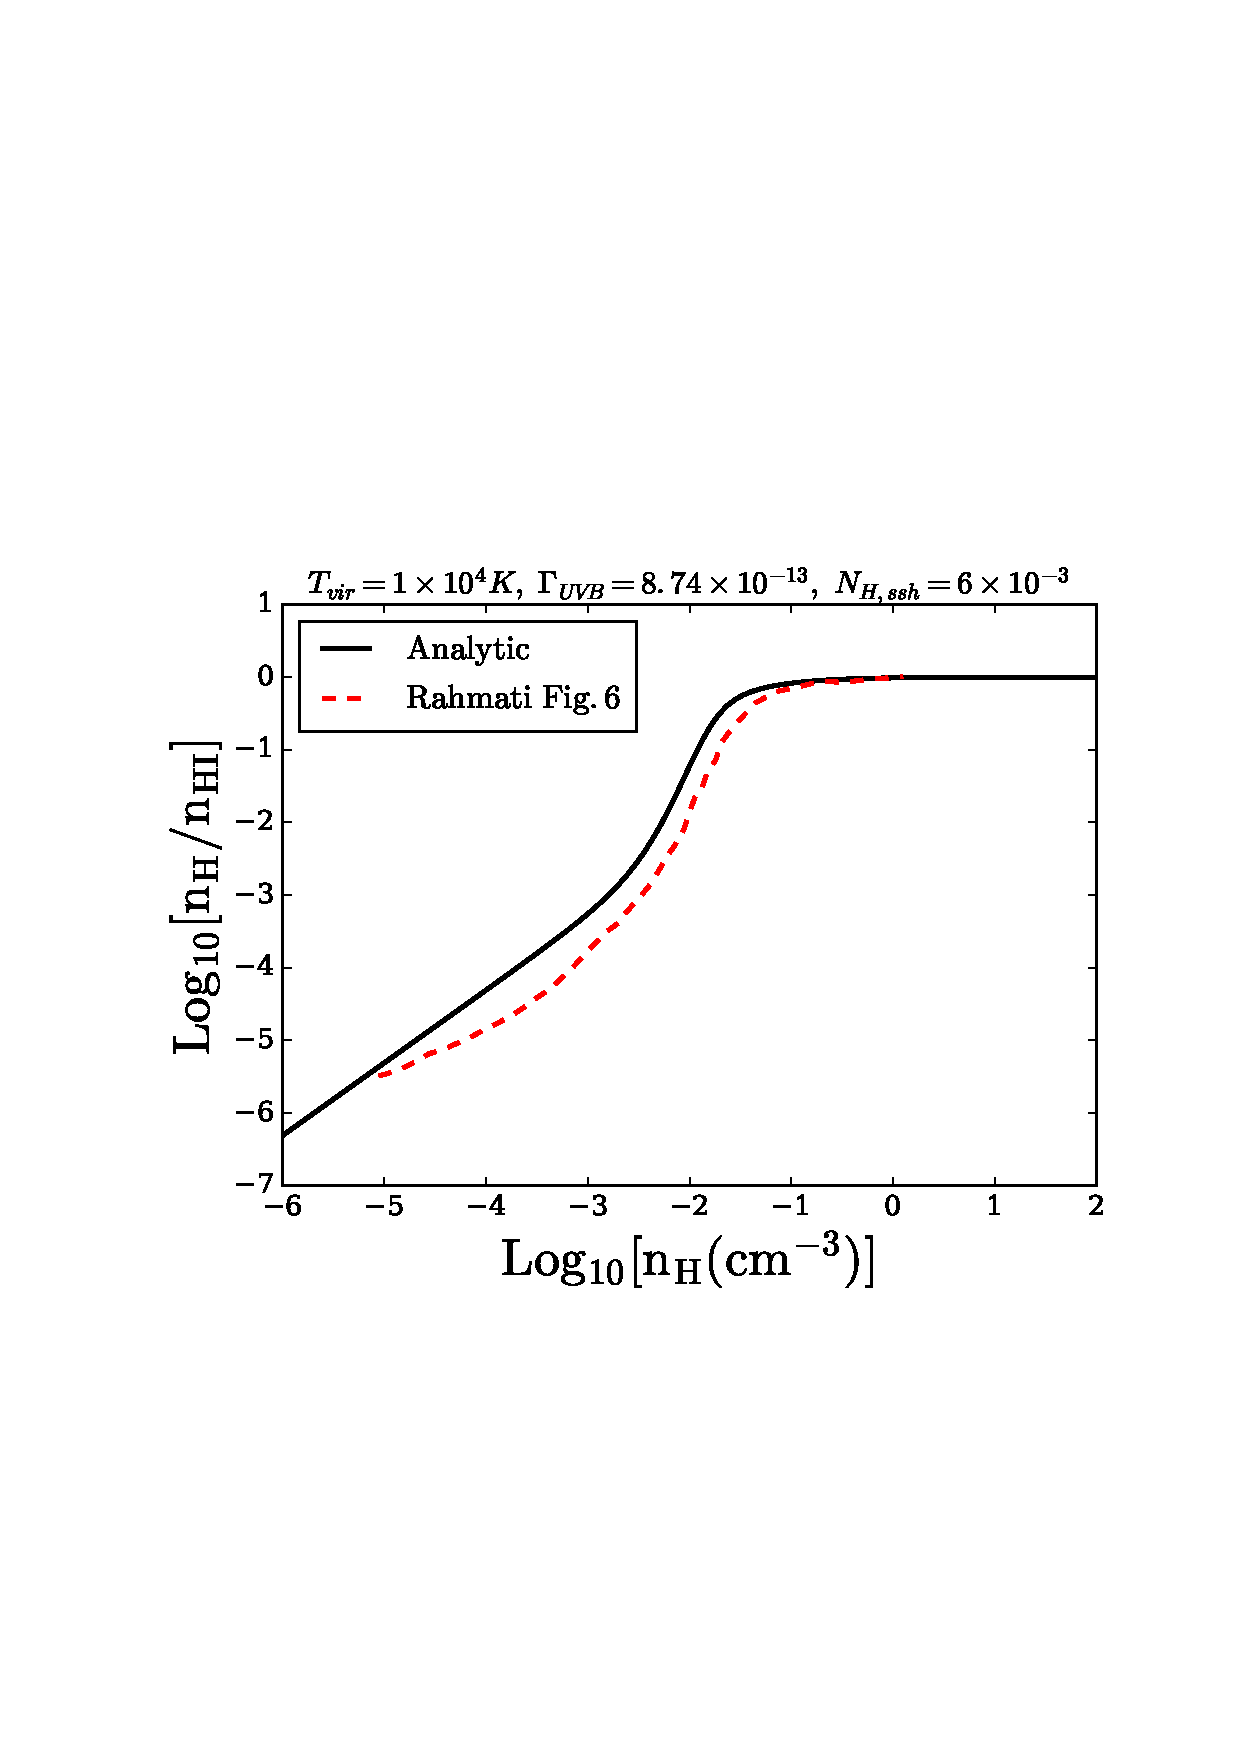
\includegraphics[scale=0.5]{../figures/nhvseta.pdf}
%\includegraphics[scale=0.5]{../code/etavsT.png}
\caption{(Up)\label{fig:eta}}
\end{figure}

\subsection{Neutral Hydrogen density profile}\label{sec:NHI}

In order to study the effect of the environment on LAEs we are
interested in the neutral Hydrogen column density.
To this aim we want to derive the neutral Hydrogen gas profile using Makino's profile
alongside the neutral hydrogen fraction derived in the previous section.

\begin{equation}
N_H = 1.6 \times 10^{21} cm^{-2} n_H^{1/2}T_4^{1/2}\left(\dfrac{f_g}{0.17} \right)
\end{equation}

Where $T_4 = T/10^{4}K$ and $f_g =\Omega_b/ \Omega_m$.

As an example we made this for a Halo of mass $M_{vir} = 1 \times
10^{12} M_{\odot}$ at $z=2$ with $r_{vir}=106kpc$ and $T =2.4\times10^{6}K$.

Left panel in figure\ref{fig:nhvsr} shows the Hydrogen density $n_H$ derived from the density $\rho$
($n_H = \rho / m_p$). The neutral hydrogen fraction $\eta$ is shown in
the middle panel. While the neutral Hydrogen profile is shown in panel
right.

%\begin{figure}[H]
%\centering
%\includegraphics[scale=0.4]{../code/nhvsr.png}
%\includegraphics[scale=0.4]{../code/etavsr.png}
%\includegraphics[scale=0.4]{../code/nhivsr.png}
%\caption{\label{fig:nhvsr}}
%\end{figure}

\section{Numerical Approach}

We trace rays of Ly$\alpha$ photons propagating in random directions, we derive
the gas properties of those halos that interact with the ray
implementing the equations described in \S \ref{sec:rho},
\S \ref{sec:NH},\S \ref{sec:eta}.\S \ref{sec:NHI}. Then we sum the column
density of every Ly$\alpha$ ray. In the following subsections we describe
these steps in detail.

\subsection{Dark Matter halo catalogue}

We use the public available data from the Illustris simulation, in particular we use
the Illustis1-dark catalogue. This is a simulation of $1820^3$ dark matter particles
with a mass of $m_{DM}=6.3 \times 10^6 M_{\odot}$ in a box of $L=106.5 Mpc$. We use
the data of halos at $z = 6.01$.

We select emitter galaxies in the range of $7 \times 10^{10} - 2
\times 10^{11} M_{\odot}$.
There are 1672 emitter halos in this mass range embedded in different
environments. In order to quantify the environment we
define the $\Delta_3$ parameter as:

\begin{equation}
\Delta_3  = \bar{r}^3 \left( \dfrac{1}{r^3} - \dfrac{1}{\bar{r}^3} \right)
\end{equation}

If $\Delta_3 < 0 $ the halo is in an over-dense environment while
if $\Delta_3 > 0 $ the halo is in an under-dense environment.

Left panel of figure \ref{fig:Halos_prop} shows the distribution of
halo mass. The right panel shows the halos environment parameter as a function
of the halo mass.

\begin{figure*}
\centering
\includegraphics[scale=0.5]{../figures/absorbers_prop.pdf}
\caption{\label{fig:Halos_prop}}
\end{figure*}

\subsection{Ray tracing}

For each emitter galaxy we follow the trajectory of a Ly$\alpha$ photon
for $10 Mpc$ in a random direction. The absorbers are selected if the
ray goes through the halo, this is when the impact parameter of the
ray $b$ is less than the virial radius of the halo.

\subsection{Column density properties and Environment}

We compute the Hydrogen density profiles using Eq.\ref{eq:rhogr}, then
we compute the Hydrogen column density using Eq.\ref{eq:NH}. Then we compute
the fraction of neutral column density $n_{HI}$ using Eq.\ref{eq:eta}.

\begin{equation}
N_H \sim 1.6 \times 10^{21} cm^{-2} n_h^{1/2}T_4^{1/2} \left(
\dfrac{f_g}{0.17}\right)^{1/2}
\end{equation}



\section{Results}

\begin{figure*}
\centering
\includegraphics[scale=0.5]{../figures/NHvsMvsD3.pdf}
\legend{\caption{}}
\end{figure*}

\begin{figure*}
\centering
\includegraphics[scale=0.5]{../figures/NHIvsMvsD3.pdf}
\end{figure*}



\bibliographystyle{mn2e}
\bibliography{references}
%begin{thebibliography}{}

%\bibitem[\protect\citeauthoryear{{Duffy}, {Schaye}, {Kay} \& {Dalla
% Vecchia}}{{Duffy} et~al.}{2008}]{Duffy2008}
%Duffy} A.~R.,  {Schaye} J.,  {Kay} S.~T.,    {Dalla Vecchia} C.,  2008,
% \mnras, 390, L64


%end{thebibliography}

\end{document}


